%\documentclass[aip,apl,english,reprint,amssymb,amsmath,graphicx]{revtex4-1}
\documentclass{article}
\usepackage[utf8]{inputenc}
\usepackage[T1]{fontenc}
\usepackage{graphicx,amssymb,amsmath}
\usepackage{mathrsfs}
\usepackage{epstopdf}
%\usepackage{natbib}
\usepackage[english]{babel}
\usepackage{xfrac}
\usepackage[section]{placeins}
%\usepackage[breaklinks=true,colorlinks=true,linkcolor=blue,citecolor=blue,urlcolor=blue]{hyperref}
\usepackage[affil-it]{authblk}
\usepackage[mincitenames=1,
maxcitenames=1,
url=false,
doi=true,
backend=biber,
style=IEEE]{biblatex}
\addbibresource{straincompensation.bib}

\usepackage[colorlinks=true]{hyperref}

\graphicspath{ {./figures/} }

\begin{document}

\title{Strain Compensation Thickness Calculator Distribution Notes}

\author{Stephen J. Polly
	\thanks{email: \texttt{\href{mailto:sjp5958@rit.edu}{sjp5958@rit.edu}}}}
	\affil{Rochester Institute of Technology, Rochester, NY 14623}
%\email{sjp5958@rit.edu}


%\affiliation{Rochester Institute of Technology -- Rochester, New York 14623 USA}

\date{\today}

\maketitle

\section{Introduction}
This program calculates the required strain compensation (SC) thickness for quantum dots (QD) and their associated wetting layer (WL). It can also be used to calculate SC thickness for quantum wells (QW), or to calculate QD volume or effective QD material coverage based on QD properties.

\section{License}

This program is free software: you can redistribute it and/or modify it under the terms of the GNU General Public License as published by the Free Software Foundation, either version 3 of the License, or (at your option) any later version.

This program is distributed in the hope that it will be useful, but WITHOUT ANY WARRANTY; without even the implied warranty of MERCHANTABILITY or FITNESS FOR A PARTICULAR PURPOSE.  See the GNU General Public License for more details.

You should have received a copy of the GNU General Public License along with this program.  If not, see \url{http://www.gnu.org/licenses/}.

The source code for this program, as well as the most recent version of this document, is available at \url{http://github.com/spolly/straincompensation}.

\section{Software Layout}

The program is divided into four sections, with some attribution at the bottom. A screenshot of the program on startup is shown in Figure \ref{fig:scexe}.

\begin{figure}
	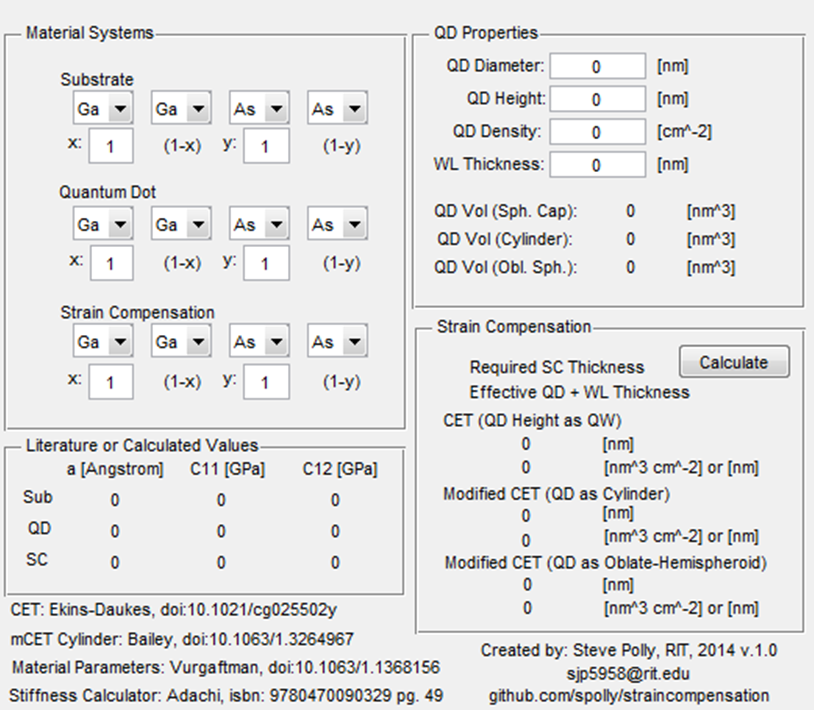
\includegraphics[width=0.85\linewidth]{scexe}
	\centering
	\caption{Screenshot of application straincompensation.m at startup.}
	\label{fig:scexe}
\end{figure}

\subsection{Material Systems}
Here the user selects the type and composition for the \texttt{Substrate}, \texttt{Quantum Dot}, and \texttt{Strain Compensation} material systems. All layers are set to GaAs by default. To select, for example, In$_{0.9}$Ga$_{0.1}$As QDs and a GaAs$_{0.17}$P$_{0.83}$ strain compensation (SC) layer: the user would select as shown in Figure \ref{fig:scexemat}. Both methods of selecting material systems shown will produce the same results.

\subsection{Literature or Calculated Values}
This section shows the lattice constant and elastic stiffness constants for the substrate, QD, and SC materials selected in the \texttt{Material System} box. If the materials are binary (e.g.: GaAs, InAs, etc.) the material parameters are taken from \citeauthor{vurgaftman_band_2001} \cite{vurgaftman_band_2001}. If they are ternaries or quaternaries, these values are calculated via methods described in Sections \ref{latticeconstant} and \ref{stiffnessconstant} for lattice constant and elastic stiffness constant, respectively.
\begin{figure}
	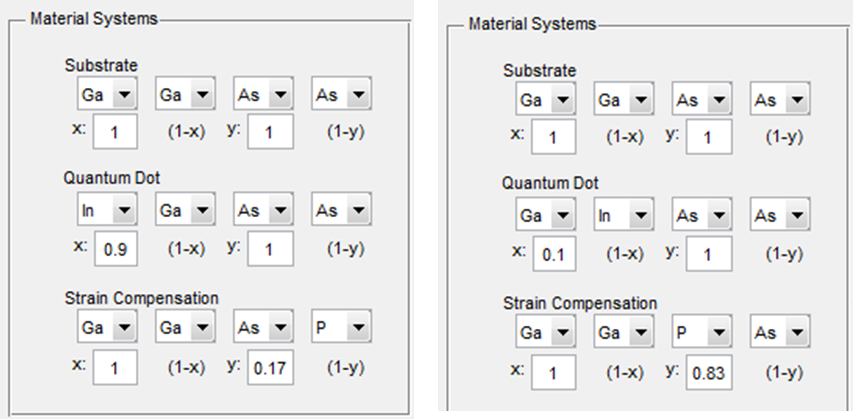
\includegraphics[width=0.85\linewidth]{scexemat}
	\centering
	\caption{Screenshot of application showing two ways of selecting the same In$_{0.9}$Ga$_{0.1}$As QD and a GaAs$_{0.17}$P$_{0.83}$ strain compensation material systems.}
	\label{fig:scexemat}
\end{figure}

\subsection{QD Properties}
In this box, the user inputs QD parameters: \texttt{QD Diameter} [nm], \texttt{QD Height} [nm], \texttt{QD Density} [cm$^{-2}$], and \texttt{WL Thickness} [nm].

This box also displays the volume of a single QD in [nm$^{3}$], based on the parameters entered, using three methods to define the QD shape: Spherical Cap, Cylinder, and Oblate-Hemispheroid. The first, \texttt{QD Vol (Sph. Cap.)} is shown here only for interest, and is not used anywhere else in the software. The other two volumes, \texttt{QD Vol (Cylinder)} and \texttt{QD Vol (Obl. Sph.)} are used in the calculation of necessary strain compensation material thicknesses using the respective Modified CET methods, described in Section \ref{straincomp}. A comparison of these QD volume methods is discussed in Section \ref{qdvolcompare}.

\subsection{Strain Compensation}
This section shows the calculated required strain compensation material thickness based on the parameters entered in the other sections. It displays the resulting SC thicknesses, as well as effective thickness, or coverage, of the QD material. This is shown in [nm$^{3}$ cm$^{-2}$] but is effectively also in units [nm]. The methods used to calculate these thicknesses are discussed in Section \ref{straincomp}.
\section{Material Parameters}

\subsection{Lattice Constants}
\label{latticeconstant}
Lattice constants of binary compounds are taken from \citeauthor{vurgaftman_band_2001} \cite{vurgaftman_band_2001}. Linear interpolation of lattice constants is done using the appropriate versions of Vegard's Law, taken from \citeauthor{adachi_band_1987} \cite{adachi_band_1987} for ternary
\begin{equation}
	\label{eq:vegardternary}
	a_{AB_{x}C_{1-x}}=x(a_{AB})+(1-x)(a_{AC})
\end{equation}
and quaternary
\begin{multline}
\label{eq:vegardquaternary}
a_{A_{x}B_{1-x}C_{y}D_{1-y}}=\\xy(a_{AC})+x(1-y)(a_{AD})
+(1-x)y(a_{BC})+(1-x)(1-y)(a_{BD})
\end{multline}
material systems.

In Equations \ref{eq:vegardternary} and \ref{eq:vegardquaternary}, \(a\) is the lattice constant, and the subscripts \(x\) and \(y\) denote the composition of the material. \(A\) and \(B\) represent group III elements while \(C\) and \(D\) are group V elements.

\FloatBarrier
\subsection{Elastic Stiffness Constants}
\label{stiffnessconstant}
Stiffness constants of binary compounds are taken from \citeauthor{vurgaftman_band_2001} \cite{vurgaftman_band_2001}. The constants of ternary and quaternary compounds are calculated using
\begin{equation}
\label{eq:adachistiffness}
ln(C_{ij})=\alpha_{ij}ln(a)+\beta_{ij}
\end{equation}
by \citeauthor{adachi_properties_2005} relating \(C_{11}\) and \(C_{12}\) to the lattice constant by a fit against measured data of binary compounds \cite[pp. 47-49]{adachi_properties_2005}. Here \(C\) is the stiffness constant, while \(i\) and \(j\) are the indices of the stiffness tensor. \(\alpha\) and \(\beta\) are coefficients extracted from a least-squares fit against experimental data.

The \(C_{11}\) and \(C_{12}\) fit \citeauthor{adachi_properties_2005} uses includes experimental values of materials (such as BN) with smaller lattice constants than for typical III-V materials used in QD research and manufacturing. This work refit \(C_{11}\) and \(C_{12}\) only for compounds with Al, Ga, and In group III elements with P, As, and Sb group V elements. This reduced the \(R^{2}\) error in matching the smaller subset of material systems used in this software. A comparison of \citeauthor{adachi_properties_2005}'s fit to the fit used here are shown in Figures \ref{fig:C11} (\(C_{11}\)) and \ref{fig:C12} (\(C_{12}\)). The coefficients from both \citeauthor{adachi_properties_2005} and This Work are shown in Table \ref{table:stiffnesscalccoeff}.

\begin{figure}
	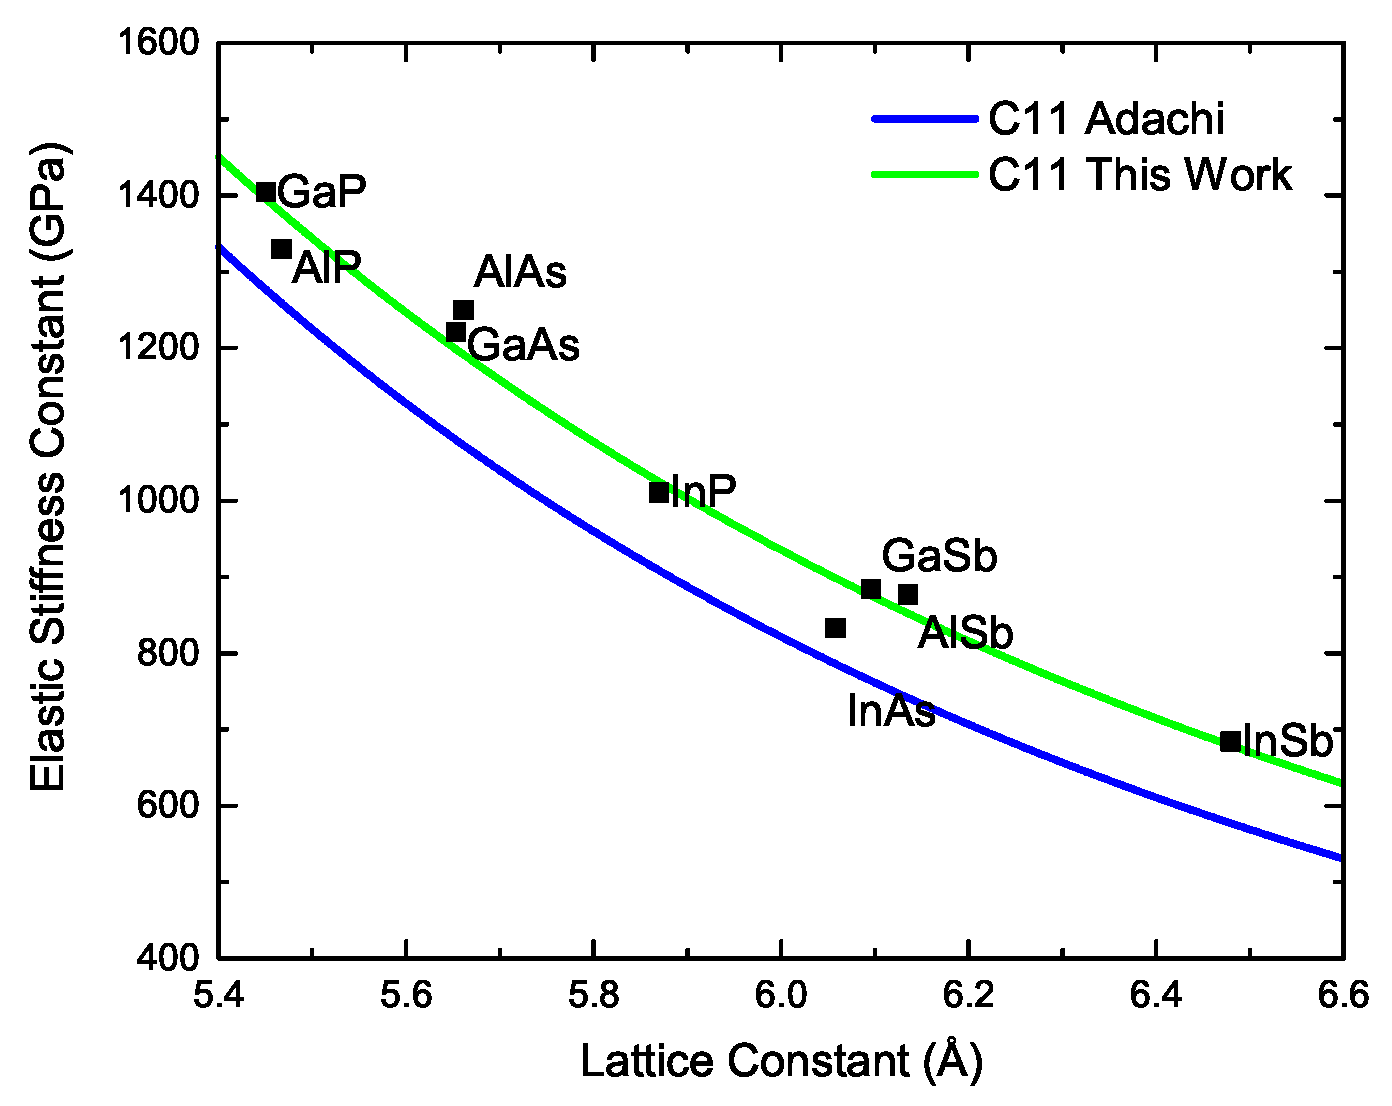
\includegraphics[width=0.85\linewidth]{C11}
	\centering
	\caption{Experimental elastic stiffness constants \(C_{11}\) from \cite{vurgaftman_band_2001} with fits by \cite{adachi_properties_2005} and this work using values in Table \ref{table:stiffnesscalccoeff} and Equation \ref{eq:adachistiffness}}
	\label{fig:C11}
\end{figure}

\begin{figure}
	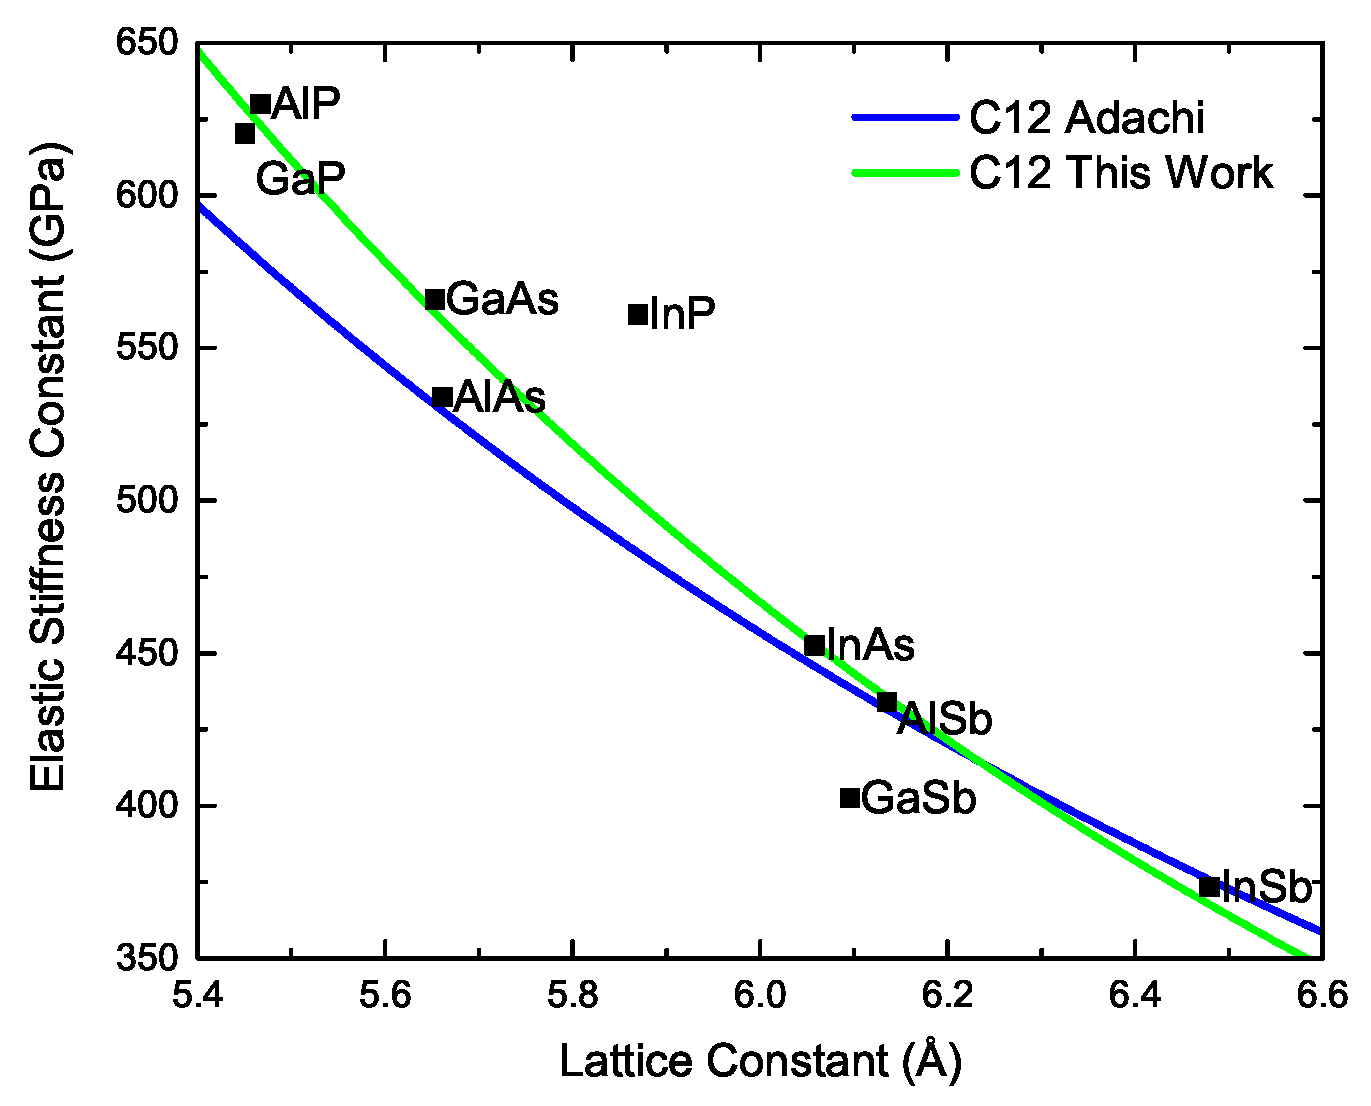
\includegraphics[width=0.85\linewidth]{C12}
	\centering
	\caption{Experimental elastic stiffness constants \(C_{12}\) from \cite{vurgaftman_band_2001} with fits by \cite{adachi_properties_2005} and this work using values in Table \ref{table:stiffnesscalccoeff} and Equation \ref{eq:adachistiffness}}
	\label{fig:C12}
\end{figure}

\begin{table}
	\caption{Equation \ref{eq:adachistiffness} Coefficients from \citeauthor{adachi_properties_2005} \cite{adachi_properties_2005} and This Work}
	\centering
	\begin{tabular}{c c c c c}
		\hline\hline
		$C_{ij}$ & \(\alpha\) (\citeauthor{adachi_properties_2005}) & \(\alpha\) (This Work) & \(\beta\) (\citeauthor{adachi_properties_2005}) & \(\beta\) (This Work) \\ % [0.5ex] % inserts table
		%heading
		\hline % inserts single horizontal line
		\(C_{11}\) & -4.59 & -4.166 & 10.33 & 9.701 \\
		\(C_{12}\) & -2.54 & -3.105 & 6.07 & 7.104 \\ %[1ex] % [1ex] adds vertical space
		\hline
	\end{tabular}
	\label{table:stiffnesscalccoeff} % is used to refer this table in the text
\end{table}
\FloatBarrier
\section{Strain Compensation Thickness}
\label{straincomp}
\subsection{Continuum Elasticity Theory (CET, QD Height as QW)}
Theory to compensate the strain of quantum wells was developed by \citeauthor{ekins-daukes_strain-balanced_2002} \cite{ekins-daukes_strain-balanced_2002}, and an explicit Equation (\ref{eq:tCET}) for the required strain compensation thickness based on this work was presented by \citeauthor{bailey_evaluation_2009} \cite{bailey_evaluation_2009}.

\begin{equation}
\label{eq:tCET}
t_{SC}=t_{QW}\frac{A_{QW}a_{SC}^{2}(a_{sub}-a_{QW})}{A_{SC}a_{QW}^{2}(a_{SC}-a_{sub})}
\end{equation}

Here, \emph{t} is a layer thickness in \AA{}, \emph{a} is a lattice constant in \AA{}, and the subscripts \emph{SC}, \emph{QW}, and \emph{sub} represent the strain compensation material, the quantum well material, and the substrate material, respectively. \emph{A} is a constant material parameter based on stiffness constants, described in Equation \ref{eq:ACET}, where \emph{i} represents the appropriate material system based on the previous set of subscripts.

In the software, these Equations are used to calculate the required strain compensation thickness for \texttt{CET (QD Height as QW)} and as part of \texttt{Modified CET (QD as Cylinder)}, though the specifics of the latter are described in the next section.

For \texttt{CET (QD Height as QW)}, the software takes the calculated material parameters, based on the user's selection, and calculates the required thickness to compensate the strain of a quantum well with a thickness equal to what the user entered into the \texttt{QD Height} field. The fields \texttt{QD Diameter}, \texttt{QD Density}, and \texttt{WL Thickness} are not used in this calculation. Consequently, the \texttt{Effective QD + QL Thickness} is identically equal to the \texttt{QD Height}.


\begin{equation}
\label{eq:ACET}
A_{i}=C_{11,i}+C_{12,i}-\frac{2C_{12,i}^{2}}{C_{11,i}}
\end{equation}
\FloatBarrier
\subsection{Modified Continuum Elasticity Theory (mCET, QD as Cylinder)}
\citeauthor{bailey_evaluation_2009} went on to modify the CET to include 3D quantum dots by introducing a weighting factor based on QD density, height, and diameter to compensate both the portion of a QD layer which is a wetting layer (WL) and that which is QDs \cite{bailey_evaluation_2009}. This method ultimately treats the QD as a cylinder, and the WL as a QW with cylinder-voids based on the density of QDs.

Two strain compensation layer thicknesses are calculated, based on Equations \ref{eq:tCET} and \ref{eq:ACET}: the first to compensate just the WL thickness (as a whole QW, Figure \ref{fig:BaileyVol}a) denoted $t_{SC,WL}$, and the second to compensate the QD (as a QW with the thickness equal to the height of the QD, Figure \ref{fig:BaileyVol}b), denoted $t_{SC,QD}$. These thicknesses are then weighted by the fractional areal density of QDs (Figure \ref{fig:BaileyVol}c), denoted by the product of $\rho$, the 2D density of QDs and $\sigma$, the cross-sectional area of the base of a single QD, calculated as the area of a circle with a diameter equal to the QD diameter. This effectively treats the QDs as cylinders (Figures \ref{fig:BaileyVol}d,e) with a volume shown by Equation \ref{eq:vQDCyl}. The full method of calculating strain compensation thickness is shown in Equation \ref{eq:mCETCyl}. It is worth being explicit here that this method treats the QD and WL as non-overlapping entities.

\begin{equation}
\label{eq:vQDCyl}
V_{QD}=\pi r^{2}h
\end{equation}

\begin{figure}
	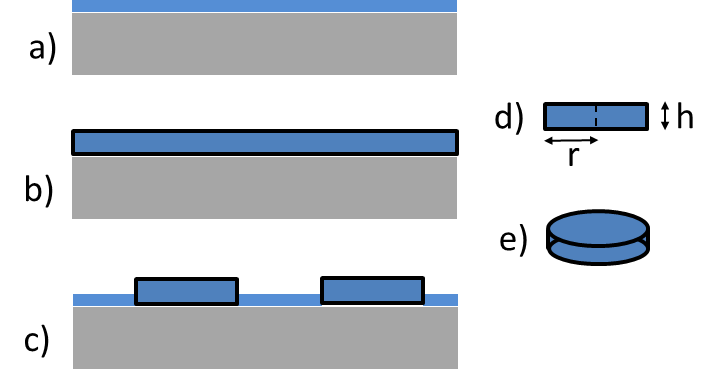
\includegraphics[width=0.95\linewidth]{QD_Bailey_cyl}
	\centering
	\caption{Visualization of the source of strain compensation calculation thickness using the modified CET presented by \citeauthor{bailey_evaluation_2009} (cylinder). a) Wetting layer thickness, b) QD thickness expanded to a QW, c) QD and WL thicknesses weighted by QD density, d) diagram of QD and e) 3D perspective.}
	\label{fig:BaileyVol}
\end{figure}

\begin{equation}
\label{eq:mCETCyl}
t_{SC,weighted}=\rho\sigma t_{SC,QD}+(1-\rho\sigma)t_{SC,WL}
\end{equation}


For \texttt{Modified CET (QD as Cylinder)}, the software takes the calculated material parameters, based on the user's selection, and calculates the required thickness to compensate the strain of a QD + WL system based on the values entered in \texttt{QD Height}, \texttt{QD Diameter}, \texttt{QD Density}, and \texttt{WL Thickness}. The volume of a single QD is shown in \texttt{QD Vol(Cylinder)} and the effective coverage of all QD material is shown in \texttt{Effective QD + WL Thickness}.
\FloatBarrier
\subsection{Modified Continuum Elasticity Theory (mCET, QD as Oblate-Hemispheroid)}

This work introduces an alternate method of determining effective QD thickness: treating the QD as half of an oblate spheroid, with a volume shown in Equation \ref{eq:vQDOblSph}. This method is similar to the weighted CET process described by \citeauthor{bailey_evaluation_2009} (see previous section) but treats the QD and the WL as overlapping entities. Again using Equations \ref{eq:tCET} and \ref{eq:ACET}, one strain compensation layer thickness is calculated for the WL (Figure \ref{fig:PollyVol}), and second a SC thickness is calculated for the effective QD thickness. This effective thickness averages the volume of a QD (as a half oblate spheroid) against the QD density through multiplication as shown in Equation \ref{eq:mCETOblSph}. Figure \ref{fig:PollyVol}d shows the origin of the shape, with Figure \ref{fig:PollyVol}e giving the parameters, and Figure \ref{fig:PollyVol}f showing the effective QD thickness multiplied by density. Figures \ref{fig:PollyVol}b-c show the evolution of how QDs are treated in this system, ultimately giving a complete QD material effective thickness.

\begin{equation}
\label{eq:vQDOblSph}
V_{QD}=\frac{\frac{4\pi}{3}r^{2}h}{2}
\end{equation}

\begin{figure}
	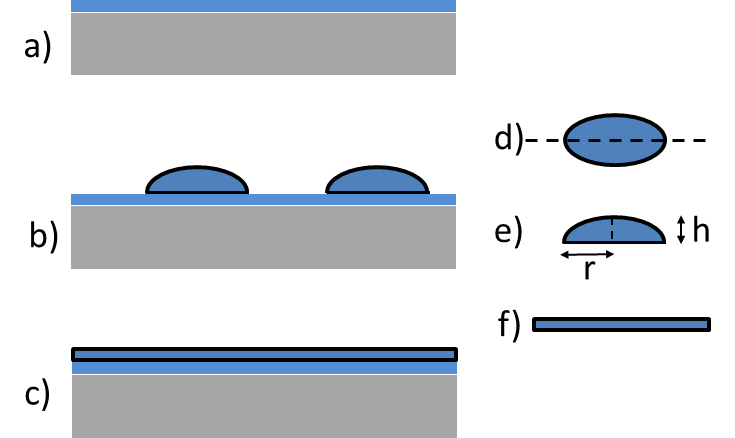
\includegraphics[width=0.95\linewidth]{QD_Polly_oblsph}
	\centering
	\caption{Visualization of the source of strain compensation calculation thickness using the modified CET presented in this work (oblate-hemispheroid). a) Wetting layer thickness, b) QDs on top of the wetting layer, c) QD thickness expanded to a QW, d) diagram of oblate spheroid with center line, e) diagram of QD and e) QD volume averaged over an area creating an effective thickness.}
	\label{fig:PollyVol}
\end{figure}

\begin{equation}
\label{eq:mCETOblSph}
t_{QD}=\frac{\frac{4\pi}{3}r^{2}h}{2}\sigma
\end{equation}

For \texttt{Modified CET (QD as Oblate-Hemispheroid)}, the software takes the calculated material parameters, based on the user's selection, and calculates the required thickness to compensate the strain of a QD + WL system based on the values entered in \texttt{QD Height}, \texttt{QD Diameter}, \texttt{QD Density}, and \texttt{WL Thickness}. The volume of a single QD is shown in \texttt{QD Vol(Obl. Sph.)} and the effective coverage of all QD material is shown in \texttt{Effective QD + WL Thickness}.
\FloatBarrier
\subsection{Comparison of QD Volume Calculation Methods}
\label{qdvolcompare}
\citeauthor{leonard_critical_1994} first described the volume of a single QD as a spherical cap \cite{leonard_critical_1994}, as shown in Equation \ref{eq:vQDLeo}. A visual explanation of this is shown in Figure \ref{fig:LeonardVol}. This volume determination is not used in any of the methods of calculating strain compensation thicknesses, and is included only for interest.

\begin{equation}
\label{eq:vQDLeo}
V_{QD}=\frac{\pi h}{6}(3r^{2}+h^{2})
\end{equation}

\begin{figure}
	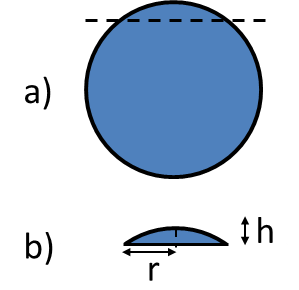
\includegraphics[width=0.35\linewidth]{QD_Leonard_sphcap}
	\centering
	\caption{QD shape made by the cap (b) of a sphere (a) as reported by \citeauthor{leonard_critical_1994} \cite{leonard_critical_1994}}
	\label{fig:LeonardVol}
\end{figure}

Comparison of the spherical cap method to the oblate-hemispheroid method is shown in Figure \ref{fig:LeoPDiff}. Over a size range typically encountered in physical QDs (height $\leq$ 5 nm, diameter $\geq$ 10 nm), these methods differ by $\sim$28\%. However, in a realm where a spherical cap no longer makes much sense (e.g.: height $>$ diameter), the spherical cap method begins to differ dramatically from the oblate-hemispheroid method (shown in Figure \ref{fig:LeoPDiff}) and the cylinder method, which is why it is not used anywhere in this software for strain compensation thickness calculations.

The percent difference between the cylinder volume and the oblate hemispheroid volume is geometric and equal to exactly 50\% \--- a cylinder has 50\% more volume than an oblate hemispheroid given the same radius and height.


\begin{figure}
	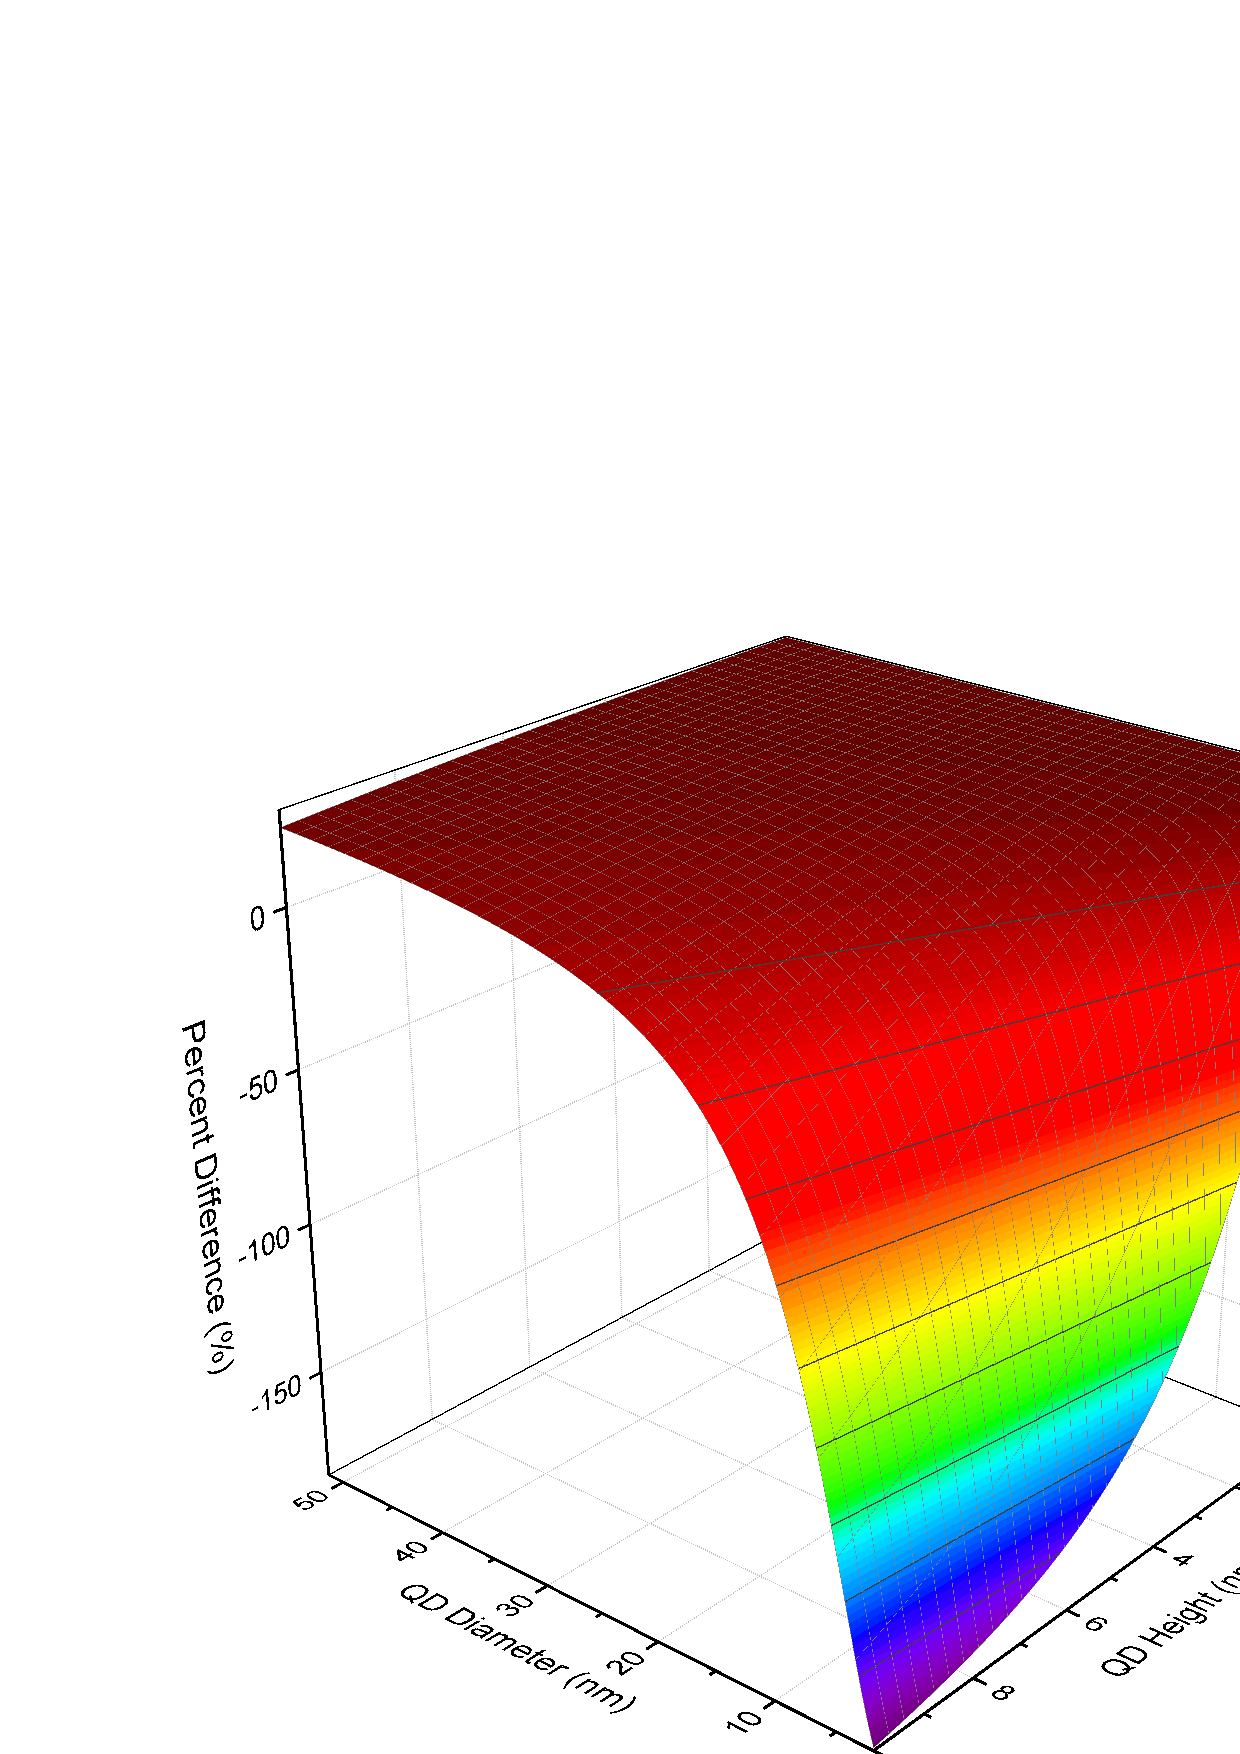
\includegraphics[width=0.900\linewidth]{Percent_Difference_QD_volume_3D}
	\centering
	\caption{Percent difference between the volumes of QDs made from spherical caps and oblate hemispheroids as a function of QD diameter and height.}
	\label{fig:LeoPDiff}
\end{figure}
\FloatBarrier

\printbibliography
\end{document}

%%% Local Variables:
%%% mode: latex
%%% TeX-master: t
%%% End:
